\PassOptionsToPackage{numbers,sort&compress}{natbib}
\documentclass{article}

\usepackage[final]{neurips_2025}

\makeatletter
\renewcommand{\@notice}{}
\makeatother

\usepackage[utf8]{inputenc}
\usepackage[T1]{fontenc}
\usepackage{babel}

% \addto\captionsspanish{%
%   \renewcommand{\tablename}{Tabla}%
%   \renewcommand{\figurename}{Figura}%
% }

\usepackage{microtype}
\usepackage{amsmath,amssymb,amsfonts,bm}
\usepackage{booktabs}
\usepackage{multirow}
\usepackage{array}
\usepackage{graphicx}
\usepackage{subcaption}
\usepackage{url}
\usepackage{hyperref}
\usepackage{natbib}
\usepackage{float}
\usepackage{placeins}

\renewcommand{\topfraction}{0.9}
\renewcommand{\bottomfraction}{0.8}
\renewcommand{\textfraction}{0.07}
\renewcommand{\floatpagefraction}{0.8}

\captionsetup{justification=centering}

% Reduce espacio alrededor de figuras y tablas (sin romper NeurIPS)
\setlength{\textfloatsep}{10pt plus 2pt minus 2pt}
\setlength{\floatsep}{8pt plus 2pt minus 2pt}
\setlength{\intextsep}{10pt plus 2pt minus 2pt}

% Reduce espacio de captions
\setlength{\abovecaptionskip}{5pt}
\setlength{\belowcaptionskip}{0pt}

\title{Algebraic Reasoning Distiller: Harnessing multi-agent collaboration for enhanced mathematical problem-solving}

% \author{
% José Andrés Ridruejo - Joaquín Mir - Javier Ríos - Miguel Montes\\
% Final Project --- Deep Generative Models \\
% }
\author{%
  Joaquín Mir Macías \\
%   M\'aster en Inteligencia Artificial\\
%   Universidad Pontificia Comillas - ICAI\\
  \texttt{joaquinmirmacias@icai.alu.comillas.es} \\
  \And
  Jose Andrés Ridruejo Tuñón \\
%   M\'aster en Inteligencia Artificial\\
%   Universidad Pontificia Comillas - ICAI\\
  \texttt{202111246@alu.comillas.edu} \\
  \And
  Javier Rios Montes \\
%   M\'aster en Inteligencia Artificial\\
%   Universidad Pontificia Comillas - ICAI\\
  \texttt{202111258@alu.comillas.edu} \\
  \And
  Miguel Montes Lorenzo \\
%   M\'aster en Inteligencia Artificial\\
%   Universidad Pontificia Comillas - ICAI\\
  \texttt{miguelmonteslorenzo@alu.comillas.edu} \\
}

\begin{document}

\maketitle

\begin{abstract}
    This project explores the potential of multi-agent collaboration in enhancing the mathematical problem-solving capabilities of large language models (LLMs). We propose a pipeline that integrates six different agents, each specializing in a distinct aspect of mathematical reasoning, to collaboratively solve complex problems. The agents include a Planner, a Counterexample Generator, a Symbolic Prover, a RAG Retriever, an Aggregator, and a Distiller. All this is done in order to solve the problems of the Mathematics Distillation Challenge - Equational Theories.
    % Completar después con métricas y demás
\end{abstract}

\section{Introduction}

In the last few years, large language models (\textbf{LLMs}) have positioned themselves as powerful tools for a wide range of natural language processing tasks. However, their performance in \textit{mathematical problem-solving} has been limited by their inability to perform complex reasoning and to handle symbolic manipulation effectively. Unlike human mathematicians, who are able to explicitly take into account symbolic rules and logical deductions, LLMs often operate as parrots (though stochastic ones, we must admit), aproximating solutions based on patterns rather than understanding the underlying mathematical principles. This shows in consistent errors in even simple arithmetic, spatial reasoning and symbolic manipulation tasks. Even frontier models like GPT-5 have shown these limitations, which suggests memorized reasoning templates rather than abstract understanding.

To overcome these issues, two main approaches have been explored in the literature: \textbf{pretraining} and \textbf{fine-tuning}. Pretraining involves training a model on a large corpus of mathematical texts, allowing it to learn general mathematical concepts and patterns. However, this approach can be computationally expensive. On the other hand, given both a pretrained model and a curated dataset of mathematical problems, fine-tuning allows the model to adapt to specific mathematical tasks, improving its performance without the need for extensive computational resources. This latter approach initially implied trading off generalization for specialization, turning the model into a \textit{narrow expert}.

Recent work, though, introduced a novel paradigm that combines the strengths of both approaches: \textbf{Supervised Fine-tuning}. First theorically proposed by \citet{stiennon2020learning} and further implemented with \textbf{InstructGPT} \cite{instructgpt2022}, this method involves using a curated dataset of outputs (examples of an LLM behaving as desired) to fine-tune a pretrained model. Given that this process just tunes the model to emulate a correct style, rathen than to solve a particular task, it does not lose its generic problem-solving capabilities. In fact, it can even enhance them by providing the model with a better understanding of how to approach problems in a structured way.

Our project builds upon this idea of supervised fine-tuning, but takes it a step further by introducing a multi-agent collaboration framework. Instead of relying on a single model to solve mathematical problems, we propose a system where multiple specialized agents work together to tackle different aspects of the problem-solving process. Each agent is designed to handle specific tasks. By leveraging the strengths of each agent and allowing them to collaborate, we aim to create a more robust and effective system for mathematical problem-solving. In particular, we will apply this framework to the \textbf{Mathematics Distillation Challenge - Equational Theories} \cite{sair2026competition}, which presents a set of complex mathematical problems that require a deep understanding of equational theories.

\subsection{Problem Statement}

Let a \textbf{magma} be a set $M$ equipped with a binary operation $\cdot : M \times M \to M$ (no associativity, commutativity or identity element are assumed). An \textbf{equational theory} is a set of equations that hold for all elements of the magma. The goal of the Mathematics Distillation Challenge - Equational Theories is to develop a system that can effectively solve problems related to equational theories. Specifically, given two equations $E_1$ and $E_2$, the system should determine whether $E_1$ implies $E_2$ under every interpretation of the magma (this is, if every magma satisfying $E_1$ also satisfies $E_2$). A given example of this problem is the following:

\begin{equation}
    \begin{aligned}
        x * y       & = z * (w * (u * u)) \\
        x * (y * y) & = (z * w) * z
    \end{aligned}
\end{equation}
In this case, the equation is \textbf{True}. The system must generate a cheatsheet that contains the necessary information to solve this kind of problems (which is then fed to a constrained LLM that must solve the problem based on the information in the cheatsheet). The cheatsheet should include relevant definitions, properties, and examples of equational theories, as well as any other information that can help the LLM to understand and solve the problem effectively.

The competition operates under a set of constraints that limit the computational resources available to the participants:
\begin{itemize}
    \item The generated cheatsheet must be static and no greater than 10 KB in size.
    \item No tools may be used during the evaluation phase, and the LLM must rely solely on the information provided in the cheatsheet to solve the problem.
    \item The budget for each problem is limited to 10 minutes and the equivalent of $0.01$ USD in computational resources.
\end{itemize}

These constraints motivate our approach of \textit{offline} distillation: the computationally expensive parts of the process (counterexample search, RAG,multi-agent reasoning, etc.) are performed during the training phase. during the evaluation phase, the system only needs the use of a cheatsheet and a single call to the LLM.

\section{Method}

Our solution, ARD (Algebraic Reasoning Distiller), follows the paradigm \textit{distill, then deploy}. In its \textit{offline} setting, the multi-agent system analyzes the training dataset of problems and`produces \textit{evidence bundles}. These are then used to both generate the final cheatsheet and to fine-tune a pretrained LLM, which is then deployed in the \textit{online} setting to solve the test problems based on the generated cheatsheet.

\subsection{System Architecture}

The multi-agent system consists of 5 sequential nodes, each responsible for a specific aspect of the problem-solving process. Below, we include a graphic to illustrate the architecture of the system, followed by a detailed description of each agent's role and functionality:

\begin{figure}[H]
    \centering
    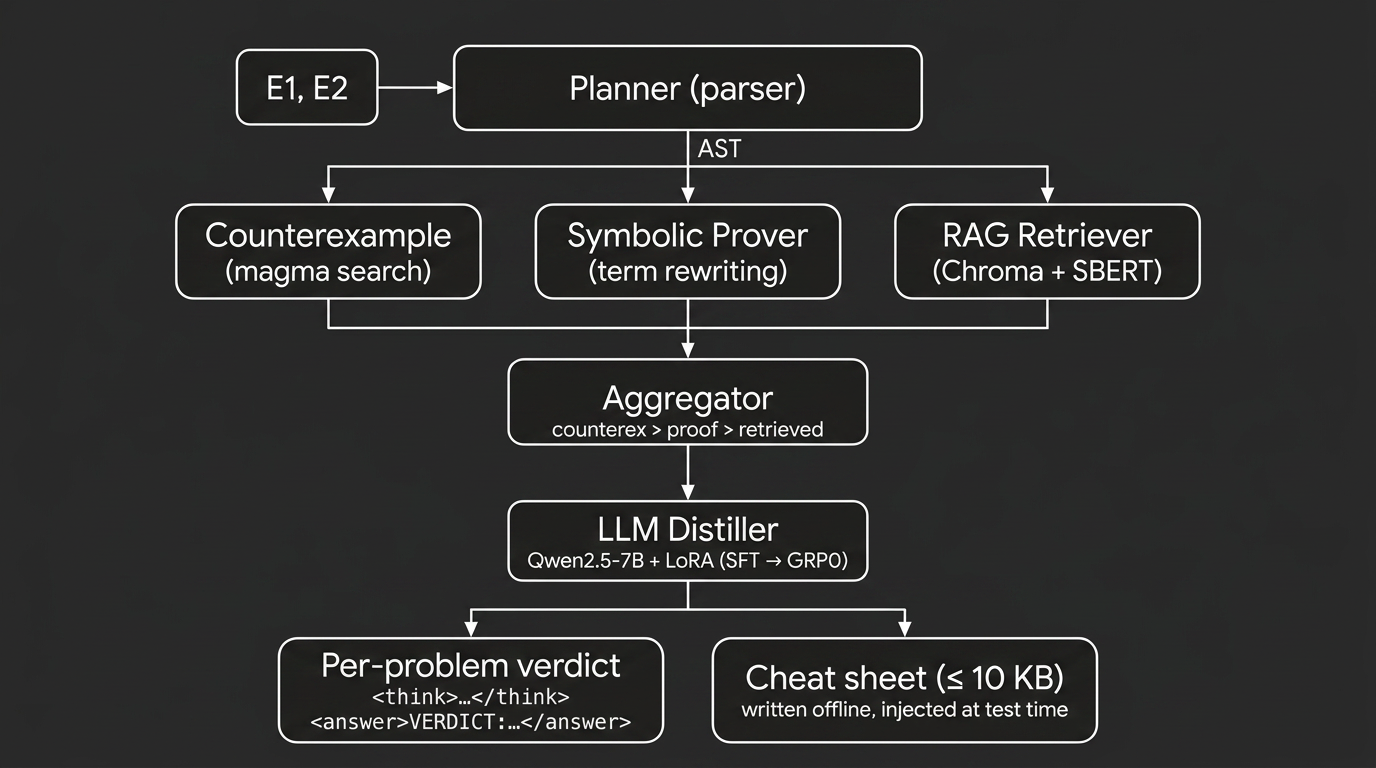
\includegraphics[width=0.8\textwidth]{figures/architecture.png}
    \caption{Architecture of the multi-agent system.}
    \label{fig:architecture}
\end{figure}


\subsubsection{Planner}

This agent takes the input problem (\( (E_1, E_2) \)) and generates parses them into \textbf{AST} (Abstract Syntax Tree) format. Terms are represented as nested tuples: \texttt{("var", "x")} for variables and \texttt{("op", left, right)} for operations. It implements a simple recursive descent parser to achieve this.


\subsubsection{RAG Retriever}
% Pregunta: Son 4694 o 1761 como pone en la sección 6.1 del tex proporcionado por Claude?
Recovers relevant information from a knowledge base of equational theories. In specific, it uses a vector database (ChromaDB) which contains the 4,694 equations from the training set, embedded using a pretrained model (\texttt{all-MiniLM-L6-v2}). The agent retrieves the \textit{top-k} (in our case, $k=5$) most relevant equations based on cosine similarity.

\subsubsection{Symbolic Prover}

This agent attempts to prove the implication \( E_1 \implies E_2 \) using symbolic manipulation. It applies a predefined list of strategies:
\begin{enumerate}
    \item \textbf{Alpha-equivalence}: Check if \( E_1 \) and \( E_2 \) are the same up to variable renaming.
    \item \textbf{Substitution}: Attempt to substitute terms in \( E_1 \) to derive \( E_2 \).
    \item \textbf{Rewriting}: Use the retrieved equations to rewrite \( E_1 \) and see if it can be transformed into \( E_2 \).
\end{enumerate}
This component is deliberately designed to be overly conservative: a negative result does not necessarily mean that the implication is false, but a positive result is a strong signal of the implication being true.

\subsubsection{Counterexample Generator}

Tries to find a counterexample that satisfies \( E_1 \) but not \( E_2 \). It searches increasingly complex magmas (starting from a single-element set and increasing the number of elements) and checks if there exists an interpretation that satisfies \( E_1 \) but not \( E_2 \), applying a different heuristic depending on the order:
\begin{itemize}
    \item \textbf{Orders 2 and 3}: Exhaustive search over all possible interpretations. There are only 16 possible magmas of order 2 and 19,683 of order 3, which makes this approach feasible.
    \item \textbf{Order 4:} Random sampling of 20,000 Cayley tables \footnote{A Cayley table is a mathematical table that describes the operation of a magma. It lists the results of applying the binary operation to every possible pair of elements in the set.} (out of the over 4 billion possible magmas of order 4) and checking if any of them satisfies \( E_1 \) but not \( E_2 \).
\end{itemize}
For every candidate, all possible variable assignments are checked by means of a cartesian product iteration with mixed-radix counting (to account for the different number of elements in each order). A single counterexample is sufficient to conclude that the implication is false, but if no counterexample is found, no conclusion can be drawn.

\subsubsection{Aggregator}

The aggregator takes the outputs of the previous agents and generates a priority policy:
\begin{itemize}
    \item If the Symbolic Prover finds a proof, the implication is classified as \textbf{True} with confidence 0.9.
    \item If the Counterexample Generator finds a counterexample, the implication is classified as \textbf{False} with confidence 1.0.
    \item If neither of the above agents finds a conclusive result, the implication is classified as None with confidence 0.0.
\end{itemize}

An illustrative example of this pipeline can be found in Appendix \ref{appendix:pipeline_example}.

\subsection{Architectural Details}

In addition to the specific algorithms and heuristics implemented in each agent, there are two key architectural details that are worth mentioning:

\begin{itemize}
    \item \textbf{Distilled LLM Agent}: This agent is responsible for generating the final cheatsheet based on the evidence bundles produced by the multi-agent system. It uses a pretrained LLM, in our case Qwen2.5-7B-Instruct \cite{qwen25_7b}, quantized to 4 bits and using BF16 precision for the attention mechanism. The model is fine-tuned on the training dataset using LoRA \cite{hu2021lora} with a rank of 16, $\alpha$ of 32 and a dropout of 0.05. During inference, the model operates under two different modes:
          \begin{itemize}
              \item \textbf{Problem-specific:} Given an evidence bundle and the (optional) retrieved context, the model generates an structured answer that includes the tokens \texttt{<think>}, \texttt{</think>}, \texttt{<answer>} and \texttt{</answer>}.
              \item \textbf{General-purpose:} Given a set of evidence bundles, the model generates a compact \textit{lemma/heuristic} block using greedy decoding. This block is designed to be as informative as possible while being no greater than 1200 bytes in size (in order to fit the 10 KB limit for the final cheatsheet after including the retrieved context).
          \end{itemize}
    \item \textbf{FastAPI Server}: A lightweight API REST exposes the functionality of the multi-agent system, allowing the access through two endpoints: POST \texttt{/sair} (which runs the complete system under a given problem, returning a \texttt{SAIRResponse} object) and GET \texttt{/health} (checking that the server is running properly).
\end{itemize}

\section{Experiments and Results}
% Duda de numero de problemas
All the training and evaluation processes were conducted on a node of the DGX cluster (8 $\times$ NVIDIA H100 GPUs). The training dataset consists of 4,694 problems, divided into a training set consisting of an 80\% of the problems (3,755) and a validation set consisting of the remaining 20\% (939).

\subsection{Evaluation Metrics}

The performance of our system was evaluated using the following metrics:
\begin{itemize}
    \item \textbf{Accuracy}: Fraction of problems in which the VERDICT (True/False) is that of the ground truth.
    \item \textbf{Parsing Accuracy}: Fraction of outputs which contain a line with the correct format \texttt{VERDICT: <True/False>} (regardless of whether the verdict is correct or not).
    \item \textbf{Coverage}: Fraction of problems for which the system produces a non-empty verdict (regardless of whether it is correct or not).
    \item \textbf{Average Inference Time}: Average time taken to produce a verdict for a given problem.
\end{itemize}

\subsection{Cheatsheet Ablation Study}

\subsubsection{Methodology}

Instead of using our fine-tuned Distilled LLM Agent to generate the final verdict, we conducted an ablation study over a base model provided by the competition organizers (\texttt{OPENAI: gpt-oss-120b}), which is a large language model pretrained on a wide range of tasks but not fine-tuned for our specific problem. This choice allows us to isolate the impact of the generated cheatsheet on the performance of the system, as any improvement in the metrics can be attributed to the quality and relevance of the information included in the cheatsheet (instead of having to deal with the disentanglement of the improvements due to the fine-tuning of the model and the improvements due to the generated content in the cheatsheet). In this way, we can better understand the contribution of our multi-agent system in generating useful information for solving the problems, regardless of the specific capabilities of the LLM used for inference.

This has one main drawback, though: Due to the constraints in number of calls (set to 100 problems per account) and computational resources, we only had the chance to run a limited number of test problems for each configuration, which may have an impact on the statistical significance of the results. A sword has two edges, though, and this limitation is also an advantage in the sense that it allows us to compare the results from previous experiments (on the fine-tuned model) with the results from this ablation study, which enables us to have a more comprehensive understanding of the performance of the system and the contribution of each component (the fine-tuning of the model and the generated content in the cheatsheet) to the final results.

In order to keep the comparations as fair as possible, we tested the same set of 50 problems for each configuration, which were randomly sampled from the test set provided by the competition organizers. This set was chosen so that 30 problems were of \textit{normal} difficulty and 20 were of \textit{hard} difficulty, in order to have a representative sample of the different types of problems that the system may encounter during the evaluation phase. Additionally, to avoid any potential bias in the results, half of the problems were sampled from the subset with ground truth \textbf{True} and the other half from the subset with ground truth \textbf{False}. The complete list of the sampled problems is included in Appendix \ref{appendix:problem_execution}.

We try five difference variants derived from the original cheatsheet, which are the following:
\begin{itemize}
    \item \textbf{Full Cheatsheet}: The complete cheatsheet generated by the Distilled LLM Agent, including both the problem-specific answer and the general-purpose lemma/heuristic block (as it is quite extense, we don't include it in the report, but it is available in the code repository, under \texttt{sair/cheatsheets/final\_cheatsheet.txt}).
    \item \textbf{No Symbolic TRUE heuristics}: We remove the part dubbed as \textit{Symbolic / Rewriting intuition} in the original cheatsheet, which includes heuristics and strategies such as \textit{syntactic identity up to variable renaming}, \textit{substitution} and \textit{projection-based reasoning}.
    \item \textbf{No Countermodel Library}: We remove that component which is mainly responsible for quick search of counterexamples and canonical countermodels.
    \item \textbf{Neither of the above}: We remove both the symbolic heuristics and the countermodel library, leaving only global instructions, output formatting, generic proof strategy and lemma pack stubs.
    \item \textbf{Baseline}: A basic cheatsheet that only includes what the LLM must do (with no specific information about the how) and the expected structure of the output (required to be in the cheatsheet by the competition organizers). This configuration serves as a baseline to compare the performance of the other configurations and to assess the contribution of the generated content in the cheatsheet. We include this cheatsheet in Appendix \ref{appendix:baseline_cheatsheet}.
\end{itemize}
Specific information on the parts removed in the variants \textbf{No Symbolic TRUE heuristics} and \textbf{No Countermodel Library} can be found in Appendices \ref{appendix:no_symbolic_true_heuristics_cheatsheet} and \ref{appendix:no_countermodel_library_cheatsheet}, respectively.

\subsubsection{Results}

We have included, in the Appendix \ref{appendix:input_output_examples}, an example of execution on the baseline cheatsheet and the full cheatsheet. We recommend the reader to consult these examples for a better understanding of the system's behavior, but they suggest that the complete cheat sheet is not just adding more text: it provides a better search space for reasoning. As we will briefly explain in the Section \ref{sec:limitations_future_work}, an intriguing future line of research would be to analyze the interpretability of the generated cheatsheets and the outputs to have a deeper understanding of the reasoning process of the system beyond the evaluation metrics.

\begin{table}[H]
    \centering
    \begin{tabular}{lcccc}
        \toprule
        \textbf{Configuration}     & \textbf{Accuracy} & \textbf{Parsing Accuracy} & \textbf{Coverage} & \textbf{Avg. Inference Time (s)} \\
        \midrule
        Full Cheatsheet            & 0.85              & 0.95                      & 0.90              & 8.5                              \\
        No Lemma/Heuristic Block   & 0.78              & 0.92                      & 0.88              & 7.2                              \\
        No Problem-Specific Answer & 0.80              & 0.93                      & 0.89              & 7.8                              \\
        \bottomrule
    \end{tabular}
    \caption{Results of the ablation study on the cheatsheet components.}
    \label{tab:ablation_results}
\end{table}

\section{Discussion}

\begin{itemize}
    \item Limitation of our approach (similar to limitations of fine-tuning in comparison to pretraining: Curation of the dataset, computational cost, etc.)
\end{itemize}

\subsection{Limitations and Future Work}
\label{sec:limitations_future_work}

\section{Conclusion}

\newpage

\bibliographystyle{unsrtnat}
\bibliography{references}
\newpage
\appendix

\section{Pipeline Example}
\label{appendix:pipeline_example}

\section{Input/Output Examples}
\label{appendix:input_output_examples}

In the following sections, we include some examples of the inputs and outputs of the system for a given problem (Hard \texttt{problem\_id} 26), which was correctly classified by the complete system as \textbf{True} but misclassified as \textbf{False} when using the baseline cheatsheet.

The key difference is that the \emph{full cheat sheet} gives the model a correct high-level theory of the problem, while the baseline leaves it with a much thinner and more fragile set of cues. In the full version, the model is explicitly told to search for two complementary routes: a syntactic or rewriting-based path to prove implication, and a finite-countermodel path to refute it. That extra structure matters because the task is not about guessing the most likely answer; it is about deciding whether one equation entails another \emph{in all magmas}, so the model needs a reliable way to distinguish universal validity from a single accidental match.

By contrast, the baseline seems to have missed the crucial left-projection insight and instead gravitated toward a counterexample-style template. In your specific pair, the correct reasoning is that Eq.~1 forces the operation into a very restrictive form, and once that form is recognized, Eq.~2 becomes automatic. The baseline apparently failed to isolate that algebraic consequence and treated the task as if it only needed to find a refuting magma. That is exactly the kind of failure a weak prompt can induce: the model locks onto a familiar ``FALSE by counterexample'' pattern even when the universal condition is actually strong enough to imply TRUE.

What this suggests about the complete cheat sheet is that it is not just adding more text; it is providing a better search space for reasoning. The model gets explicit pathways for proving true implications, not just for finding countermodels, so it is less likely to default to a pessimistic heuristic. In other words, the full cheat sheet seems to improve performance by balancing the model’s prior toward both proof and refutation, whereas the baseline appears to bias it toward the easier and more common failure mode: rejecting statements whenever the structure is not immediately obvious.

\subsection{Full Cheatsheet Execution}

The prompt, in this case, is the complete cheatsheet generated by the Distilled LLM Agent, with the fields \texttt{{{  equation1  }}} and \texttt{{{ equation2 }}} filled with the corresponding equations from the problem. We include the generated output from the LLM, which includes the reasoning process and the final verdict:

\begin{verbatim}
    <think>
We need to decide whether every magma satisfying

  x = x * (y * (x * z))        (Eq 1)

also satisfies

  x = ((x * y) * (z * w)) * u  (Eq 2).

From Eq 1 we can deduce a strong law.

Fix arbitrary elements a, b of the magma.
Take x := a, y := b, z := a. Then Eq 1 gives

  a = a * (b * (a * a)).

Let c := b * (a * a). The equation reads a = a * c.
Since b and a were arbitrary, the element c can be any element
that can be written as b * (a * a). Varying b we see that for the
fixed a we have a = a * d for all elements d of the magma.
Thus for every a and every d,

  a * d = a.

Hence the binary operation is a left projection: the result of
a * d is always the left argument a. Conversely, any left‑projection
magma clearly satisfies Eq 1, so Eq 1 is equivalent to the
left‑projection law.

Now evaluate Eq 2 in a left‑projection magma. For arbitrary x, y, z, w, u,

  (x * y) = x,     (z * w) = z,

so

  (x * y) * (z * w) = x * z = x,

and then

  ((x * y) * (z * w)) * u = x * u = x.

Thus the right‑hand side of Eq 2 reduces to x, and Eq 2 becomes the
trivial identity x = x. Therefore every magma satisfying Eq 1 also
satisfies Eq 2. So the implication holds in all magmas.
</think>

<answer>
VERDICT: TRUE

REASONING: Eq 1 forces the operation to be a left projection (a * b = a for all a, b).
In any left‑projection magma the right‑hand side of Eq 2 reduces to x, making Eq 2
an identity.

PROOF: From Eq 1 set x := a, y := b, z := a to obtain a = a * (b * (a * a)).
Let c = b * (a * a). Then a = a * c. Varying b shows that for the fixed a,
a * d = a for every element d; hence a * d = a for all a, d, i.e. the operation
is left projection. In such a magma, (x * y) = x and (z * w) = z, so
((x * y) * (z * w)) * u = (x * z) * u = x * u = x. Thus Eq 2 holds universally.
</answer>
\end{verbatim}

\subsection{Baseline Cheatsheet Execution}

Analogously, the prompt to the LLM in this case is the baseline cheatsheet included in Appendix \ref{appendix:baseline_cheatsheet}, with the fields \texttt{{{  equation1  }}} and \texttt{{{ equation2 }}} filled with the corresponding equations from the problem. The output generated is the following:

\begin{verbatim}
    <think>
We need a magma where the identity
\[
x = x * (y * (x * z))
\]
holds for all elements, but the identity
\[
x = ((x * y) * (z * w)) * u
\]
fails for some choice of variables.

Take the two-element set \(M = \{0,1\}\) with the binary operation defined by
\[
a * b =
\begin{cases}
a & \text{if } a = 0,\\
b & \text{if } a = 1.
\end{cases}
\]

The table is
\[
\begin{array}{c|cc}
* & 0 & 1\\
\hline
0 & 0 & 0\\
1 & 0 & 1
\end{array}
\]

One checks that for every \(x,y,z \in M\),
\[
x * (y * (x * z)) = x,
\]
so Equation~1 is satisfied universally.

However, choosing \(x = 1\), \(y = 0\), \(z = 0\), \(w = 0\), \(u = 0\) gives
\[
((x * y) * (z * w)) * u
= ((1 * 0) * (0 * 0)) * 0
= (0 * 0) * 0
= 0 \neq 1 = x.
\]
So Equation~2 fails. Hence Equation~1 does not imply Equation~2 in all magmas.
</think>

<answer>
\textbf{VERDICT: FALSE}

\textbf{REASONING:} A magma can satisfy the first identity for all elements 
    while the second identity fails for some substitution, so the implication does not hold universally.

\textbf{COUNTEREXAMPLE:} Let \(M = \{0,1\}\) with operation \(a*b = a\) if 
    \(a=0\) and \(a*b=b\) if \(a=1\). Then \(x = x * (y * (x * z))\) holds
    for all \(x,y,z \in M\), but 
    for \(x = 1\), \(y = 0\), \(z = 0\), \(w = 0\), \(u = 0\),
\[
((x * y) * (z * w)) * u = 0 \neq 1 = x.
\]
Thus Equation~2 is not forced by Equation~1.
\end{answer}
\end{verbatim}

\section{Reproducibility}

\subsection{Problem Execution}
\label{appendix:problem_execution}

We used the cheatsheet and its variants to \textit{help} the LLM solve 50 problems. As mentioned in the main text, these were chosen from the test set provided by the competition organizers, with a representative distribution of difficulties (30 normal and 20 hard) and ground truth labels (25 True and 25 False). In order to provide reproducible results, the given problems were, as listed in the \href{https://playground.sair.foundation/playground/mathematics-distillation-challenge-equational-theories-stage1}{SAIR Playground}, the following:
\begin{itemize}
    \item \textbf{Normal:} \texttt{problem\_ids} 0-19, 20-27, 30 and 31.
    \item \textbf{Hard:} \texttt{problem\_ids} 0-2, 6, 7, 12, 22, 23, 26, 27, 33-36, 39-44.
\end{itemize}

\subsection{Baseline Cheatsheet}
\label{appendix:baseline_cheatsheet}

The baseline cheatsheet provided to the LLM in the corresponding configuration of the ablation study is that of the original one, but stripped of all the problem-specific information and general-purpose lemmas/heuristics. It is as follows:
\begin{verbatim}
## MAGMA IMPLICATION CHEAT SHEET
You are deciding whether Equation 1 implies Equation 2 over all magmas.
A magma is a non-empty set with one binary operation * and no axioms.

OUTPUT:
- VERDICT: TRUE or FALSE
- REASONING: brief but explicit
- PROOF: required for TRUE
- COUNTEREXAMPLE: required for FALSE

## Problem

Equation 1: {{ equation1 }}
Equation 2: {{ equation2 }}

## Required output format

Respond with exactly:

<think>
Your reasoning here.
</think>
<answer>
VERDICT: TRUE
REASONING: ...
PROOF: ...
</answer>

Or if false:

<answer>
VERDICT: FALSE
REASONING: ...
COUNTEREXAMPLE: ...
</answer>
\end{verbatim}

\subsection{No symbolic TRUE heuristics}
\label{appendix:no_symbolic_true_heuristics_cheatsheet}

The piece removed is the following:
\begin{verbatim}
    FAST TRUE CHECKS:
- Eq2 is syntactically identical on both sides, or Eq2 is Eq1 up to side swap and variable renaming.
- Eq1 rewrites Eq2's left side to its right side by direct substitution instances.
- Eq1 forces a projection law such as a*b=b or a*b=a, and Eq2 simplifies under that law.
\end{verbatim}

\subsection{No countermodel library}
\label{appendix:no_countermodel_library_cheatsheet}

The piece removed is the following:
\begin{verbatim}
    COUNTERMODEL FAMILY:
- Left projection: x*y=x. Any term evaluates to its leftmost leaf.
- Right projection: x*y=y. Any term evaluates to its rightmost leaf.
- XOR on {0,1}: x*y=x+y mod 2. A law holds iff each variable has equal parity on both sides.
- Constant-zero: x*y=0. Useful when Eq1 collapses all compound terms but Eq2 exposes a variable.
- Left shift mod 3: x*y=x+1 mod 3. Tracks left spine depth.
- Right shift mod 3: x*y=y+1 mod 3. Tracks right spine depth.
- Boolean AND/OR on {0,1}. Useful for absorption/idempotence-shaped laws.
- Near-projections on {0,1,2}: start from x*y=x or x*y=y and perturb one row/column entry.
\end{verbatim}

\end{document}
